\documentclass[11pt,a4paper]{article}
\usepackage[utf8]{inputenc}
\usepackage[T1]{fontenc}
\usepackage{mathpazo}
\usepackage[scaled=0.92]{helvet}
\usepackage{microtype}
\usepackage[a4paper,margin=1.9cm,top=1.7cm,bottom=1.9cm]{geometry}
\usepackage{amsmath,amssymb}
\usepackage[export]{adjustbox}
\usepackage{graphicx}
\usepackage{booktabs}
\usepackage{caption}
\usepackage{enumitem}
\usepackage{array}
\usepackage[hidelinks]{hyperref}

\captionsetup{font=small,labelfont=bf}
\setlist{nosep,leftmargin=1.4em}
\setlength{\parskip}{0.35em}
\setlength{\parindent}{0pt}
\AtBeginDocument{\setlength{\abovedisplayskip}{5pt}\setlength{\belowdisplayskip}{5pt}%
  \setlength{\abovedisplayshortskip}{3pt}\setlength{\belowdisplayshortskip}{3pt}}
\setlength{\textfloatsep}{10pt}\setlength{\intextsep}{8pt}
\graphicspath{{fig/}}
\newcommand{\og}{«~}
\newcommand{\fg}{~»}
\newcolumntype{L}[1]{>{\raggedright\arraybackslash}p{#1}}
\renewcommand{\abstractname}{Résumé}
\renewcommand{\refname}{Références}
\renewcommand{\figurename}{Figure}
\renewcommand{\tablename}{Tableau}

\title{\textbf{Détection de contours par chemin minimal}\\[0.3em]
\large D'après la méthode de Cohen \& Kimmel (1997)}
\author{Dov Costa--- M1, Traitement d'image}
\date{Octobre 2026}

\begin{document}
\maketitle
\vspace{-1.5em}

% ===========================================================================
\section{À quoi sert la méthode ?}

Délimiter le contour d'un objet dans une image est une tâche de base en imagerie : mesurer un organe sur
une IRM, suivre un vaisseau sanguin, détourer une pièce mécanique. Le faire à la main, pixel par pixel, est
long ; le faire de façon entièrement automatique demande souvent des milliers d'images annotées.

La méthode de Cohen \& Kimmel \cite{cohen97} propose un intermédiaire : l'utilisateur \textbf{clique
quelques points} sur le bord de l'objet, et l'algorithme trace tout seul le contour entre ces points, en
suivant les bords de l'image. Elle a trois atouts : le résultat est le \emph{meilleur possible} (minimum
global), le tracé est \emph{continu}, et elle ne demande \emph{aucun apprentissage}.

Dans ce projet, nous avons implémenté la méthode en Python, puis nous l'avons appliquée à deux bases
d'images médicales : les vaisseaux de la rétine et le cœur en IRM.

% ===========================================================================
\section{Le problème : un problème d'optimisation}

Entre deux points cliqués $p_0$ et $p_1$, il existe une infinité de courbes possibles. On veut celle qui
suit le mieux les bords de l'image. On donne donc un \og prix\fg{} $\tilde P(x)$ à chaque pixel $x$, faible
sur les bords, et on cherche la courbe la moins chère :
\begin{equation}
  \min_{C} \; E(C) = \int_C \tilde P\big(C(s)\big)\, ds
  \qquad \text{avec } C(0) = p_0 \text{ et } C(L) = p_1 .
\end{equation}
La fonction coût $E$ additionne les prix des pixels traversés ; la contrainte impose que la courbe relie les
deux points cliqués. Le contour cherché est donc un \textbf{chemin minimal}, comme le trajet le plus rapide
entre deux villes sur une carte routière.

% ===========================================================================
\section{La méthode, étape par étape (exemple de l'engrenage)}

\subsection*{Étape 1 : la carte de coût}

L'image est en niveaux de gris : chaque pixel $x$ a une \textbf{intensité} $I(x)$ entre 0 (noir) et 1
(blanc) ; une image en couleur est d'abord convertie en gris. Un bord est un endroit où l'intensité
change brusquement. On le mesure par le \textbf{gradient} $\nabla I = (g_x, g_y)$, c'est-à-dire la
variation d'intensité entre pixels voisins, horizontalement ($g_x$) et verticalement ($g_y$), calculée
avec les filtres de Sobel. Sa norme $\|\nabla I\| = \sqrt{g_x^2 + g_y^2}$ est grande sur un bord net et
nulle dans une zone uniforme. 

Le prix $\tilde P(x)$ d'un pixel $x$ se définit alors par :
\begin{equation}
  \tilde P(x) = \frac{1}{1 + \alpha\, g(x)} + w,
  \qquad g(x) = \frac{\|\nabla I(x)\|}{\max \|\nabla I\|},
\end{equation}
où :
\begin{itemize}
  \item $\tilde P(x)$ : prix (coût) du pixel $x$, faible sur un bord ;
  \item $g(x) \in [0,1]$ : force du bord en $x$ (norme du gradient divisée par sa valeur maximale dans
        l'image) ; $g \approx 1$ sur un bord net, $g \approx 0$ dans une zone uniforme ;
  \item $\alpha > 0$ : contraste entre bord et fond (un pixel de bord coûte environ $1+\alpha$ fois moins cher) ;
  \item $w > 0$ : paramètre de régularisation, prix minimal de chaque pixel (il pénalise la longueur du
        chemin).
\end{itemize}
Sur un bord, $\tilde P \approx w$ (presque gratuit) ; ailleurs, $\tilde P \approx 1 + w$.

\begin{figure}[!htb]
  \centering
  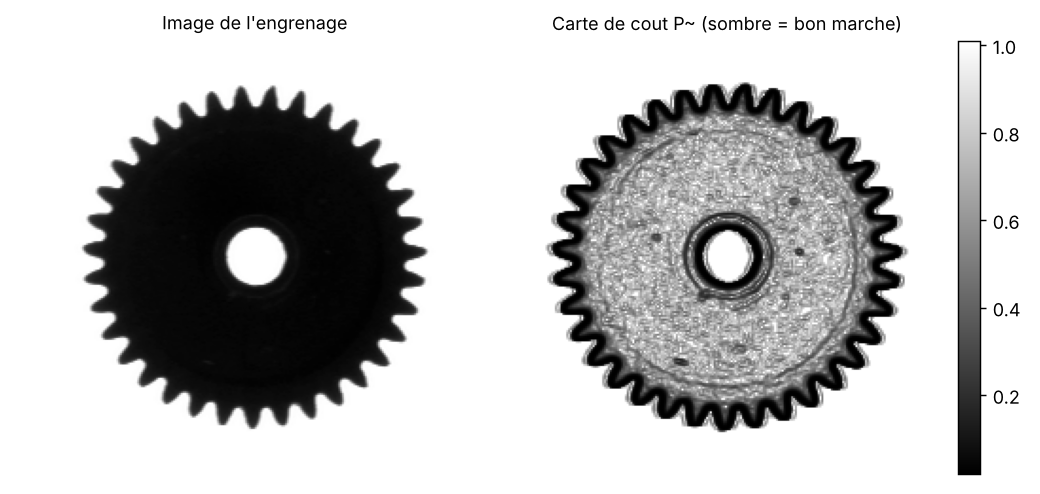
\includegraphics[width=0.72\linewidth]{engrenage_image_cout.png}
  \caption{L'engrenage (gauche) et sa carte de coût (droite) : le bord des dents est sombre, donc bon marché.}
  \label{fig:cout}
\end{figure}

\subsection*{Étape 2 : le Fast Marching (calcul du coût de tous les chemins)}

Entre $p_0$ et $p_1$, il existe une \textbf{infinité de chemins} possibles : on ne peut pas tous les essayer
pour garder le moins cher. L'idée de Cohen et Kimmel est de changer de point de vue : au lieu de chercher
directement le chemin, on calcule d'abord, pour \emph{chaque} pixel $x$, le coût du meilleur chemin qui
le relie à $p_0$. On note ce coût $U(x)$.

On peut se représenter $U$ comme \textbf{l'heure d'arrivée d'un feu} allumé en $p_0$ : le feu avance vite
là où le prix est faible (sur les bords) et lentement ailleurs. Traverser un pixel prend un temps égal à son
prix, ce qui s'écrit avec l'\emph{équation eikonale} :
\begin{equation}
  \|\nabla U(x)\| = \tilde P(x), \qquad U(p_0) = 0 .
\end{equation}

Le \textbf{Fast Marching} résout cette équation en faisant avancer le front du feu pixel par pixel
(figure~\ref{fig:propagation}) :
\begin{enumerate}[nosep,leftmargin=*]
  \item au départ, seul $p_0$ est brûlé, avec $U(p_0)=0$ ;
  \item parmi les pixels du front, on fige celui qui a le plus petit $U$ (sa valeur ne changera plus) ;
  \item on met à jour ses quatre voisins, puis on recommence jusqu'à atteindre $p_1$.
\end{enumerate}
Pour mettre à jour un voisin, on note $a$ la plus petite valeur de $U$ déjà connue à sa gauche ou à sa
droite, et $b$ celle en haut ou en bas. Sa nouvelle valeur $u$ est la solution de
$(u-a)^2 + (u-b)^2 = \tilde P^2$ (version discrète de l'équation eikonale) :
\begin{equation}
  u = \begin{cases}
    \min(a,b) + \tilde P & \text{si } |a-b| \ge \tilde P \quad \text{(le feu arrive d'un seul côté),}\\[3pt]
    \tfrac12\Big(a + b + \sqrt{2\tilde P^2 - (a-b)^2}\Big) & \text{sinon (il arrive des deux côtés).}
  \end{cases}
\end{equation}
Le second cas fait la différence avec l'algorithme de Dijkstra : le feu peut avancer en diagonale et le
front reste bien rond. Avec un prix constant, notre $U$ retrouve la distance à vol d'oiseau à 1,3 pixel
près, alors que Dijkstra se trompe jusqu'à 41\,\% en diagonale. Grâce à une file de priorité, le calcul
coûte $O(N\log N)$ pour $N$ pixels.

\begin{figure}[!htb]
  \centering
    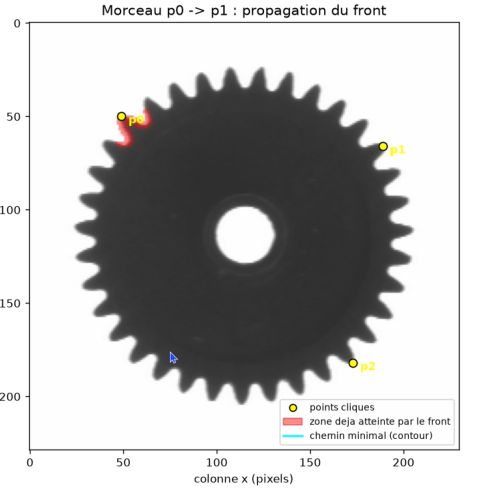
\includegraphics[width=0.29\linewidth,trim=0 0 0 18,clip]{fig/propagation1.png}\hspace{0.02\linewidth}
  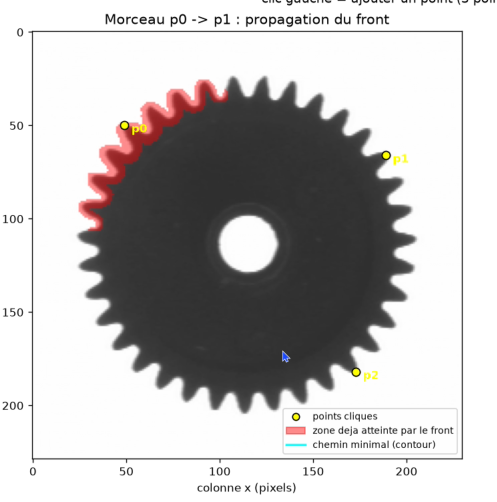
\includegraphics[width=0.29\linewidth,trim=0 0 0 18,clip]{fig/propagation2.png}\hspace{0.02\linewidth}
  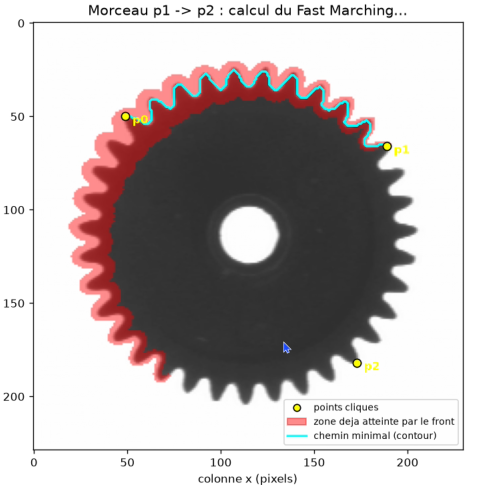
\includegraphics[width=0.29\linewidth,trim=0 0 0 18,clip]{fig/propagation3.png}
  \caption{Propagation du front sur l'engrenage, à trois instants successifs (en rouge : pixels déjà
    atteints). Le feu part de $p_0$ et court le long du bord, où le prix est faible ; une fois $p_1$
    atteint, le chemin minimal (cyan) est extrait, puis on repart de $p_1$ vers $p_2$.}
  \label{fig:propagation}
\end{figure}



\subsection*{Étape 3 : retrouver le chemin (backtracking)}

$U$ vaut 0 en $p_0$ et augmente partout autour. Il suffit donc de partir de $p_1$ et de \textbf{descendre la
pente de $U$} :
\begin{equation}
  \frac{dC}{ds} = -\nabla U(C(s))
  \qquad\Longrightarrow\qquad
  x_{k+1} = \text{voisin de } x_k \text{ (parmi 8) de plus petit } U .
\end{equation}
On arrive forcément en $p_0$, par le chemin le moins cher. Pour un contour fermé, on clique $n$ points $p_0, p_1, \dots, p_{n-1}$ sur le bord. On calcule le chemin
minimal entre chaque point et le suivant, puis entre le dernier et le premier pour fermer le contour.
Sur l'engrenage (4 clics, figure~\ref{fig:engrenage}), le contour est formé de 4 chemins mis bout à bout :
\[
  p_0 \to p_1, \qquad p_1 \to p_2, \qquad p_2 \to p_3, \qquad p_3 \to p_0 .
\]

\begin{figure}[!htb]
  \centering
  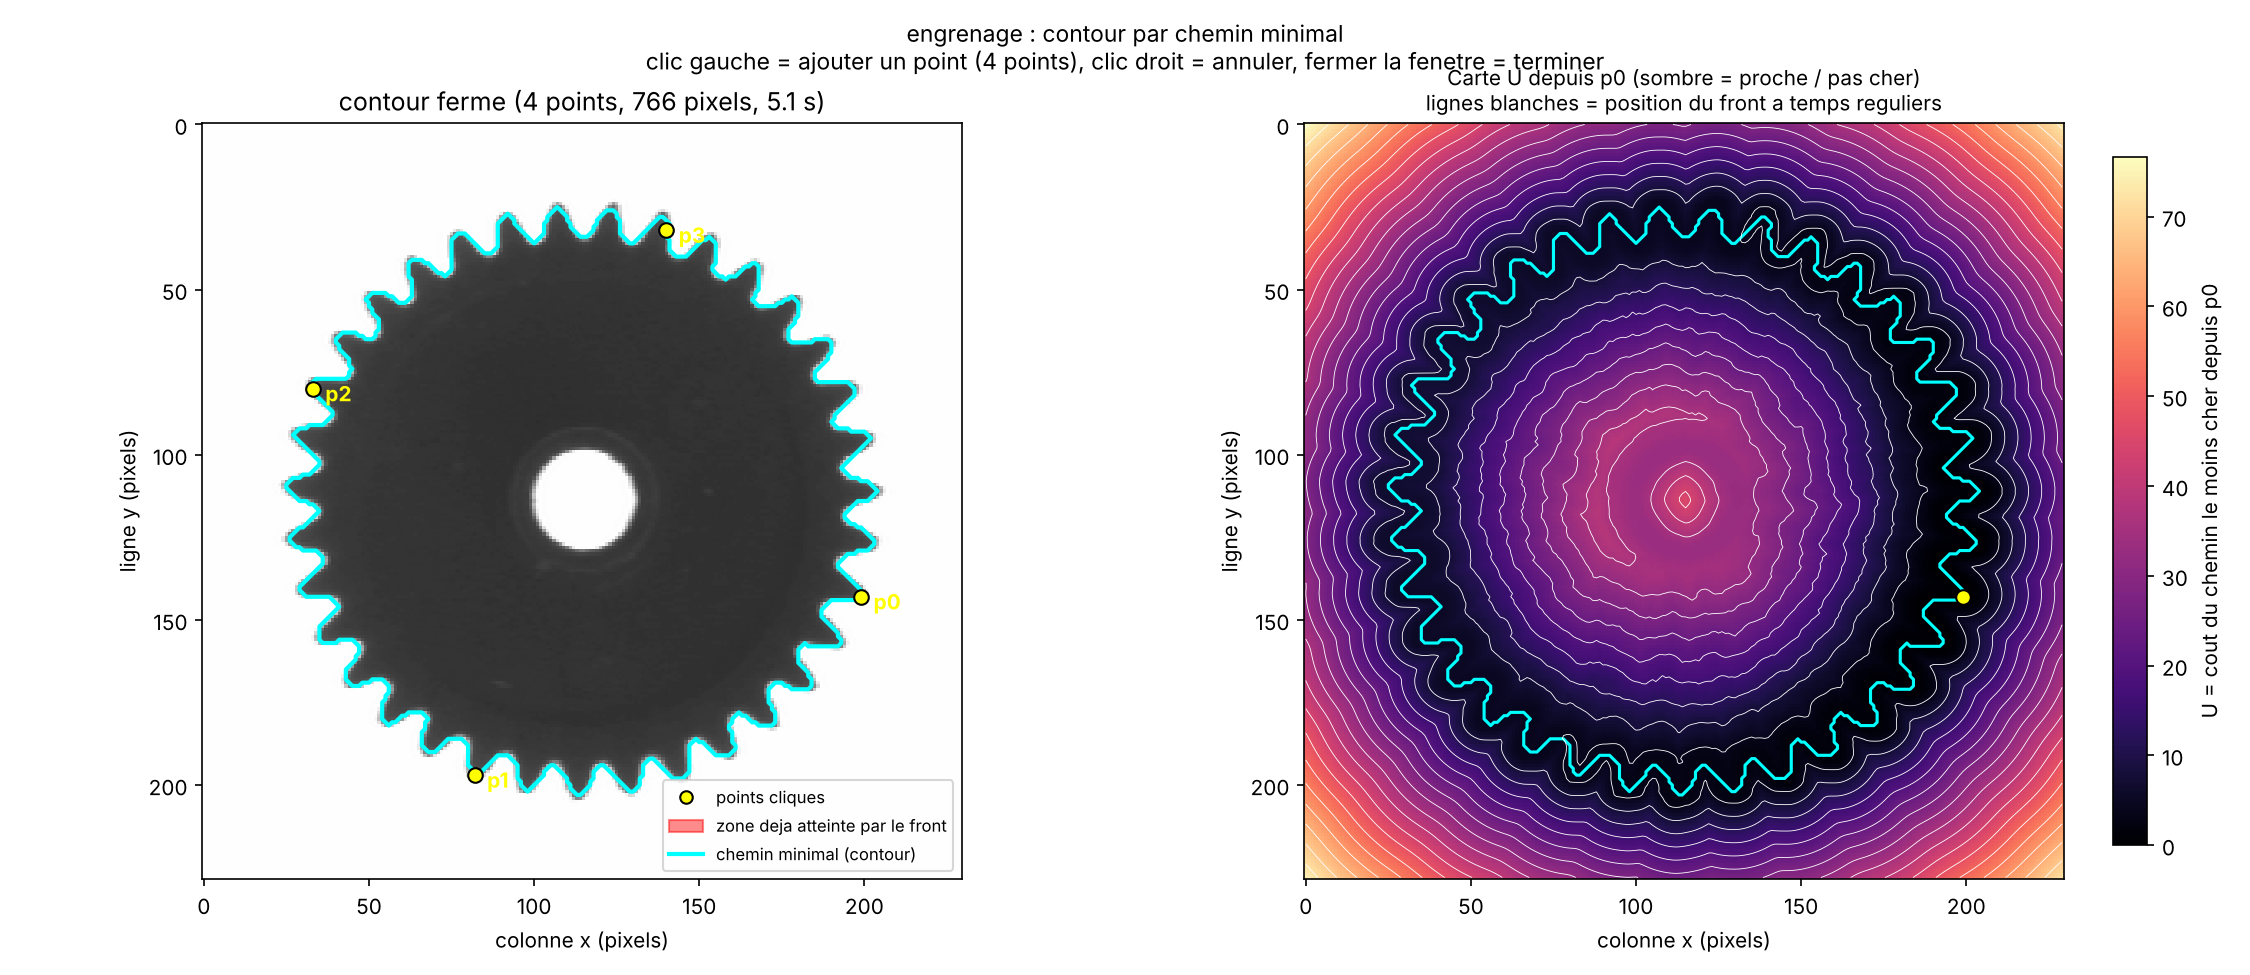
\includegraphics[width=0.62\linewidth]{engrenage_fm.png}
  \caption{Résultat sur l'engrenage avec 4 clics (p0 à p3). Gauche : le contour suit toutes les dents.
  Droite : la carte $U$ depuis p0 ; les lignes blanches sont les positions du feu à temps réguliers, il
  file le long du bord.}
  \label{fig:engrenage}
\end{figure}

\subsection*{Le réglage de $w$}

Avec les mêmes clics, on fait varier $w$ seul (figure~\ref{fig:w}). Un petit $w$ suit tous les détails ; un
grand $w$ préfère les chemins courts et coupe les dents dès $w = 0{,}5$. \textbf{Le bon réglage dépend du
but} : suivre des détails fins, ou obtenir une forme lisse et robuste au bruit.

\begin{figure}[!h]
  \centering
  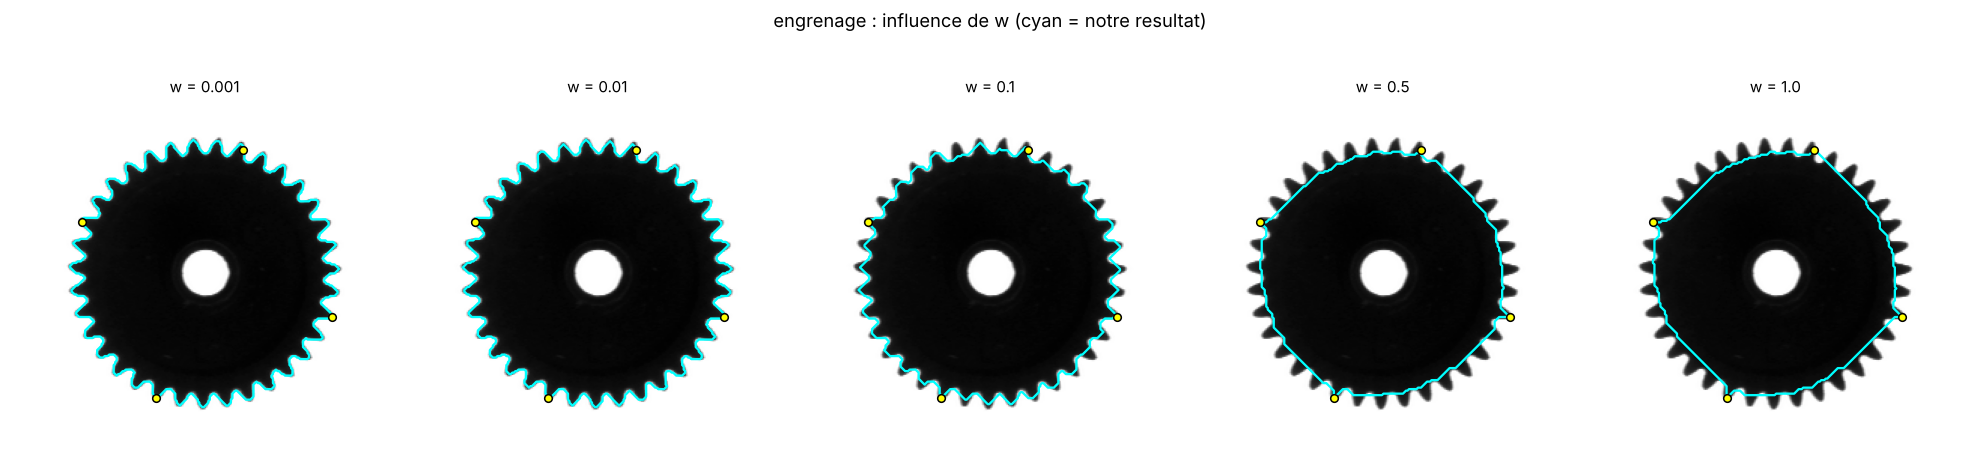
\includegraphics[width=0.82\linewidth]{w_engrenage.png}
  \caption{Mêmes clics, $w$ de 0,001 à 1 : plus $w$ est grand, plus le contour coupe les dents.}
  \label{fig:w}
\end{figure}

% ===========================================================================
\section{Application aux bases de données médicales}

Pour savoir si la méthode marche vraiment, on la compare à une \textbf{vérité terrain} : le tracé
d'un expert, sur deux bases d'images publiques.

\subsection{Le cœur en IRM (base ACDC)}

La base ACDC \cite{bernard18} fournit des IRM du cœur avec le contour du ventricule gauche tracé par un expert.
On y applique exactement la méthode de l'engrenage : carte de coût par gradient et contour fermé par clics.
On mesure l'accord avec le score de \textbf{Dice} (égal au F1-score) :
\begin{equation}
  \text{Dice} = \frac{2\,|A \cap B|}{|A| + |B|} \in [0, 1],
\end{equation}
où $A$ est la zone entourée par notre contour et $B$ celle de l'expert (1 = superposition parfaite).
Sur la coupe médiane du patient 001, \textbf{6 clics} autour du ventricule donnent un \textbf{Dice de 0,91}
(figure~\ref{fig:irm}) ; sur les 18 coupes du patient, le Dice reste entre 0,89 et 0,91. La partie manquante
correspond aux \emph{muscles papillaires} : notre chemin suit le bord le plus net et passe devant eux, alors
que l'expert les inclut dans la cavité.

\begin{figure}[!htb]
  \centering
  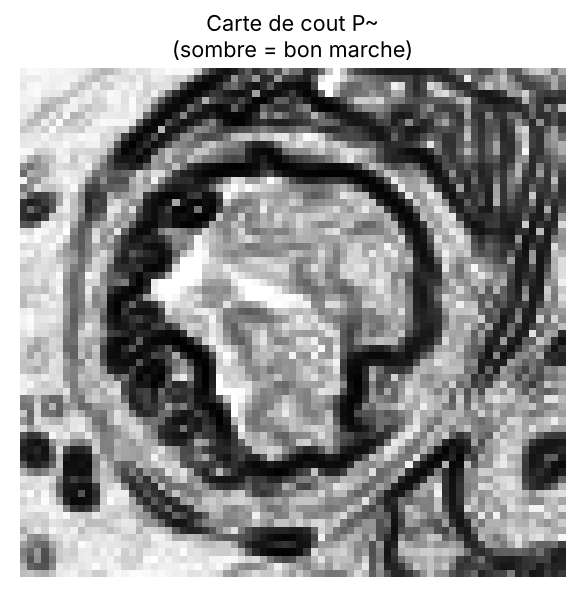
\includegraphics[height=4.7cm,valign=b]{irm_cout.png}\hspace{4mm}
  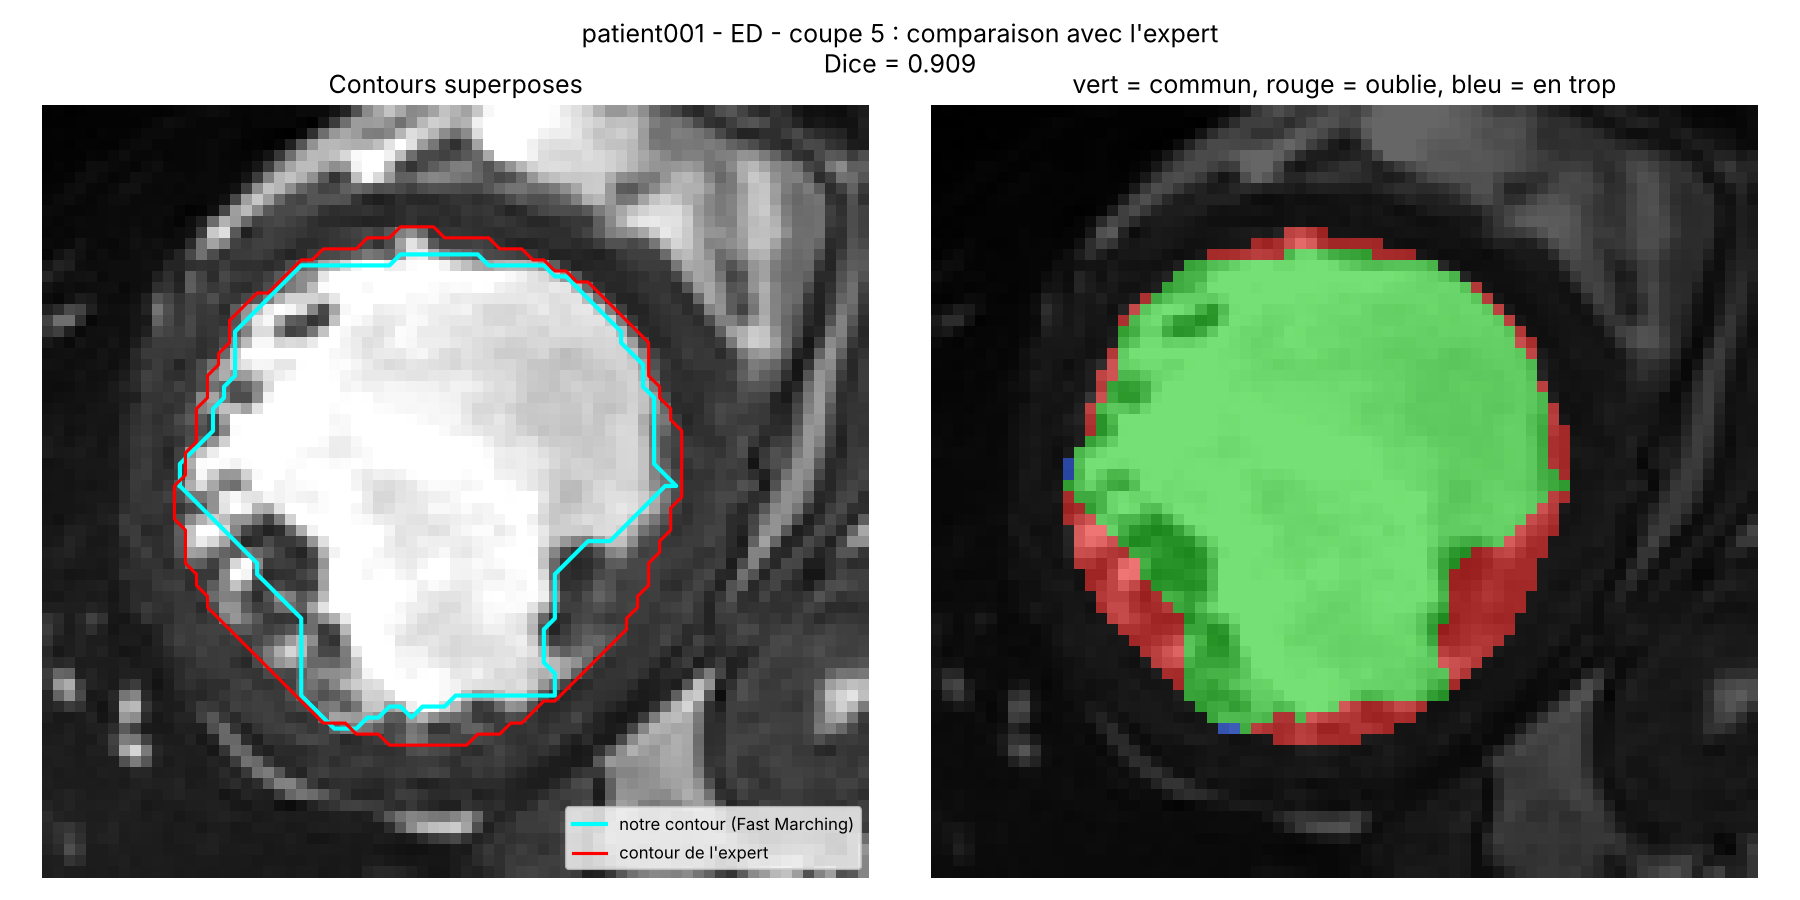
\includegraphics[height=4.9cm,valign=b]{irm_eval.png}
  \caption{IRM du ventricule gauche (zoom). Gauche : la carte de coût, où le bord du ventricule est sombre.
  Milieu : notre contour (cyan) et celui de l'expert (rouge). Droite : pixels communs (vert), oubliés
  (rouge, les muscles papillaires), en trop (bleu).}
  \label{fig:irm}
\end{figure}

\textbf{Suivi pendant un battement.} L'IRM \og ciné\fg{} filme le cœur : 30 images par battement. On clique
6 points sur la première image ; ensuite, à chaque image, chaque point glisse le long de son rayon vers le
bord le plus proche (avec une pénalité s'il saute trop loin, car le cœur bouge peu d'une image à l'autre), et
le Fast Marching retrace le contour. Le suivi ne dérive pas : \textbf{Dice de 0,906 en diastole} (cœur rempli)
\textbf{et 0,887 en systole} (cœur contracté), et la contraction mesurée, 17\,\% d'aire, est la même que
celle de l'expert.
\textbf{Animation :} \href{https://drive.google.com/file/d/1AEJK4vhxZayERtE9HWirIwNcTwk1bDqs/view?usp=sharing}{\underline{voir le GIF du battement}}.

\begin{figure}[!htb]
  \centering
  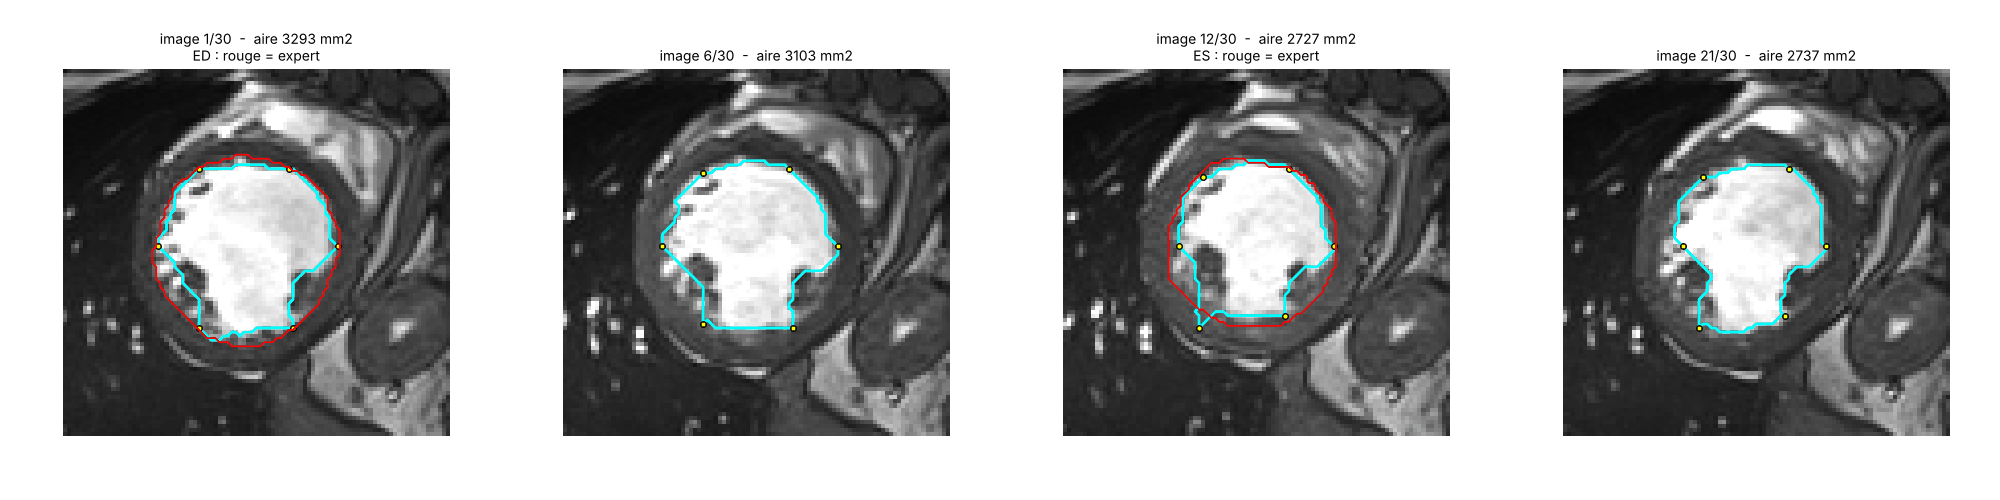
\includegraphics[width=0.56\linewidth,valign=c]{coeur_images.png}\hfill
  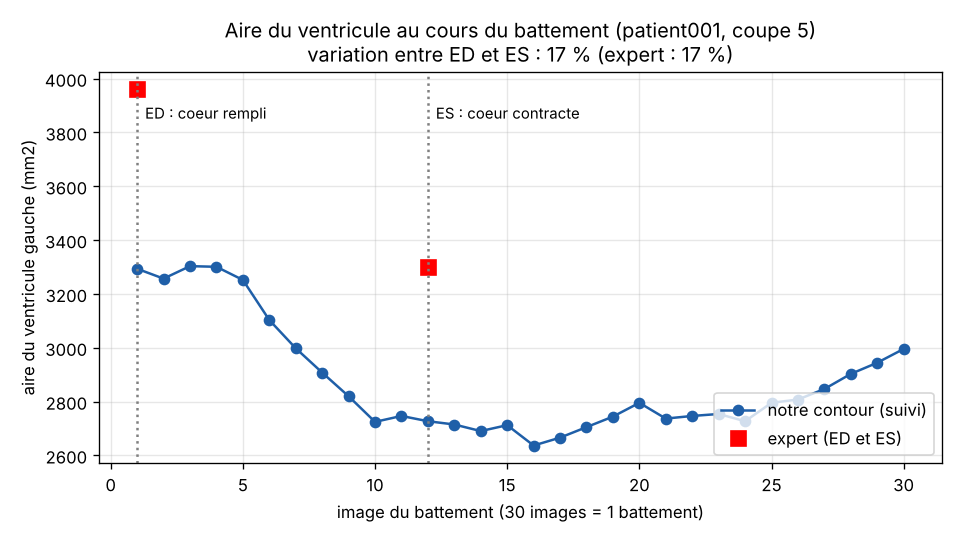
\includegraphics[width=0.42\linewidth,valign=c]{aire.png}
  \caption{Gauche : images 1, 6, 12 et 21 du battement, avec le contour suivi (cyan) et l'expert (rouge).
  Droite : aire du ventricule au cours du battement ; notre aire est environ 17\,\% plus petite (muscles
  papillaires), mais elle varie comme celle de l'expert.}
\end{figure}

\clearpage

\subsection{Les vaisseaux de la rétine (base DRIVE)}

On cherche maintenant à suivre un \textbf{vaisseau sanguin} de la rétine entre deux points cliqués. La base
DRIVE \cite{staal04} contient 40 photos de fond d'œil, et pour chacune, un expert a tracé tous les vaisseaux
à la main (figure~\ref{fig:oeil_base}).

\begin{figure}[!htb]
  \centering
  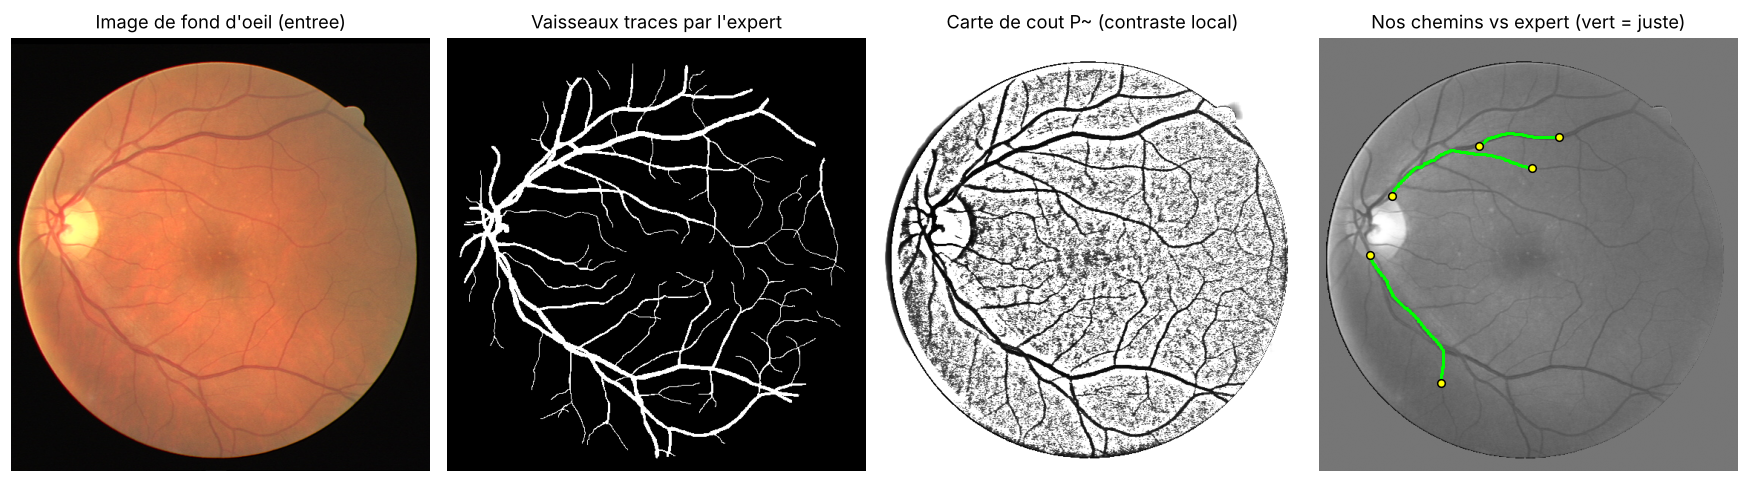
\includegraphics[width=0.86\linewidth]{oeil_21_base.png}
  \caption{Image 21 de DRIVE. De gauche à droite : la photo, les vaisseaux tracés par l'expert, notre carte de
    coût où les vaisseaux sont noirs, et nos chemins comparés à l'expert : vert = juste, rouge = faux.}
  \label{fig:oeil_base}
\end{figure}

La démarche est la même que pour l'engrenage et le cœur :
\begin{enumerate}[nosep,leftmargin=*]
  \item on construit la carte de coût de l'image ;
  \item on clique deux points sur un vaisseau ;
  \item le Fast Marching calcule $U$, puis le backtracking trace le chemin minimal ;
  \item on compare ce chemin aux vaisseaux tracés par l'expert.
\end{enumerate}
Seule la carte de coût change. Le chemin doit suivre le centre du vaisseau, qui est plus sombre que le tissu
qui l'entoure. On utilise donc une carte de coût fondée sur le \textbf{contraste local} :
\begin{equation}
  v(x) = \max\big(0,\; \bar I(x) - I(x)\big), \qquad
  \tilde P(x) = \frac{1}{1 + \alpha\, v(x)/\max v} + w,
\end{equation}
où $I(x)$ est l'intensité de l'image (canal vert de la photographie, le plus contrasté), $\bar I(x)$ sa
moyenne sur un carré de $21 \times 21$ pixels autour de $x$, et $v(x)$ le contraste local, grand au centre
d'un vaisseau.

\textbf{Évaluation sur les 40 images.} Le test est automatisé, avec des \textbf{paramètres fixés pour toutes
les images} : $\alpha = 100$ et $w = 0{,}01$. Sur chaque image, le programme tire au hasard 3 paires de
points dans les vaisseaux de l'expert, à la place des clics, et trace le chemin entre chaque paire. On
obtient ainsi 120 chemins.

\textbf{Mesure.} Un chemin est une ligne, et non une zone : le Dice ne s'applique donc pas. Pour chaque
chemin, on mesure plutôt la \textbf{part de ses pixels qui tombent dans un vaisseau de l'expert}. Un score de
100\,\% signifie que le chemin ne sort jamais du vaisseau.

\textbf{Comparaison des cartes de coût.} Pour vérifier que le contraste local est le bon choix, on refait
exactement le même test, sur les mêmes 120 paires de points, avec d'autres cartes de coût : celle par
gradient utilisée pour l'engrenage, et une carte par intensité où un pixel sombre est bon marché. Le
tableau~\ref{tab:drive} donne, pour chaque carte, le score moyen sur les 120 chemins et la proportion de
chemins presque parfaits (score supérieur à 99\,\%).

\begin{table}[!h]
  \centering\small
  \begin{tabular}{lcc}
    \toprule
    Carte de coût & Score moyen & Chemins presque parfaits ($> 99\,\%$) \\
    \midrule
    Gradient (celle de l'engrenage) & 85,5\,\% & 16\,\% \\
    Intensité & 63,5\,\% & 13\,\% \\
    Contraste local, $\alpha = 30$ & 97,2\,\% & 80\,\% \\
    \textbf{Contraste local, $\alpha = 100$} & \textbf{98,9\,\%} & \textbf{90\,\%} \\
    \bottomrule
  \end{tabular}
  \caption{Part des chemins qui reste dans les vaisseaux de l'expert, sur les 40 images de DRIVE.}
  \label{tab:drive}
\end{table}

Le contraste local est nettement le meilleur : \textbf{98,9\,\%} de chaque chemin reste en moyenne dans un
vaisseau, et 90\,\% des chemins sont presque parfaits. La carte par gradient suit les deux bords du vaisseau
plutôt que son centre, et celle par intensité est trompée par l'éclairage non uniforme. Les rares échecs du
contraste local sont des raccourcis entre deux branches proches.

% ===========================================================================
\clearpage
\section{Comparaison avec des méthodes récentes et limites}

\begin{table}[!htb]
  \centering\small
  \begin{tabular}{L{3.1cm}L{0.9cm}L{5.4cm}L{2.2cm}L{3.2cm}}
    \toprule
    Méthode & Année & Principe & Apprentissage & Lien avec ce travail \\
    \midrule
    Cohen \& Kimmel \cite{cohen97} & 1997 & Chemin minimal, Fast Marching & aucun & méthode étudiée \\
    Chen et al.\ \cite{chen17} & 2017 & Chemin minimal avec courbure & aucun & évite les raccourcis \\
    DeepIGeoS \cite{wang19} & 2019 & Réseau de neurones + distance géodésique & oui & réutilise $U$ \\
    nnU-Net \cite{isensee21} & 2021 & Réseau U-Net automatique, sans clic & oui (beaucoup) & référence sur ACDC \\
    MedSAM \cite{ma24} & 2024 & Grand modèle, une boîte autour de l'objet & oui (1,6 M) & segmentation guidée \\
    \bottomrule
  \end{tabular}
  \caption{Positionnement face à des méthodes récentes (comparaison à partir des articles).}
\end{table}

Les méthodes d'apprentissage profond sont plus précises et automatiques (nnU-Net atteint un Dice de l'ordre de
0,95 sur le ventricule gauche d'ACDC), mais elles demandent des centaines d'images annotées et une carte
graphique, et on ne sait pas toujours expliquer leurs résultats. Le chemin minimal donne au contraire un
résultat garanti et explicable, sans aucune donnée. Ses limites, observées dans ce projet : le réglage de $w$
et de la carte de coût, les raccourcis entre deux bords proches, la dépendance aux clics, et un contour qui
suit le bord le plus net plutôt que la convention de l'expert.

% ===========================================================================
\section{Conclusion}

Avec un seul algorithme et sans aucun apprentissage, nous avons détouré un engrenage, détouré le ventricule
gauche (Dice $\approx 0{,}91$), suivi le cœur pendant un battement et suivi les vaisseaux de la rétine
(98,9\,\% sur 40 images). Le Fast Marching garantit le chemin le moins cher, mais la qualité du résultat
dépend entièrement de la \textbf{carte de coût}, que nous avons construite à la main pour chaque type
d'image, et du réglage de $w$.

Trois pistes permettraient d'aller plus loin :
\begin{itemize}[nosep,leftmargin=*]
  \item \textbf{Apprendre la carte de coût.} Au lieu de choisir sa formule à la main, un réseau de neurones
    entraîné sur les images annotées prédirait, pour chaque pixel, s'il est sur un bord ou un vaisseau. Le Fast
    Marching tracerait ensuite le chemin entre les clics, comme aujourd'hui.
  \item \textbf{Pénaliser la courbure} \cite{chen17}, pour des contours plus lisses qui ne suivent pas chaque
    creux, comme celui des muscles papillaires.
  \item \textbf{Passer en 3D :} le Fast Marching s'étend directement aux volumes IRM.
\end{itemize}

% ===========================================================================
\small
\begin{thebibliography}{9}
\setlength{\itemsep}{0pt}
\bibitem{cohen97} L.~D. Cohen, R.~Kimmel. Global minimum for active contour models: a minimal path
  approach. \emph{Int.\ J.\ Computer Vision}, 24(1):57--78, 1997.
\bibitem{chen17} D.~Chen, J.-M. Mirebeau, L.~D. Cohen. Global minimum for a Finsler elastica minimal path
  approach. \emph{Int.\ J.\ Computer Vision}, 122(3):458--483, 2017.
\bibitem{wang19} G.~Wang et al. DeepIGeoS: a deep interactive geodesic framework for medical image
  segmentation. \emph{IEEE TPAMI}, 41(7):1559--1572, 2019.
\bibitem{isensee21} F.~Isensee et al. nnU-Net: a self-configuring method for deep learning-based biomedical
  image segmentation. \emph{Nature Methods}, 18:203--211, 2021.
\bibitem{ma24} J.~Ma et al. Segment anything in medical images. \emph{Nature Communications}, 15, 2024.
\bibitem{bernard18} O.~Bernard et al. Deep learning techniques for automatic MRI cardiac multi-structures
  segmentation and diagnosis: is the problem solved? \emph{IEEE Trans.\ Medical Imaging}, 37(11), 2018.
\bibitem{staal04} J.~Staal et al. Ridge-based vessel segmentation in color images of the retina.
  \emph{IEEE Trans.\ Medical Imaging}, 23(4):501--509, 2004.
\end{thebibliography}
\normalsize

% ===========================================================================

\end{document}
